\section{Sistema proposto}
\begin{frame}{Sistema de arquivos distribuído com RAID}
	
	\begin{columns}
		\column{0.55\textwidth}
		\begin{itemize}
			\item Desenvolvido em linguagem Java.
			\item Pode se escolher a forma de armazenamento entre RAID 0, RAID 1 e RAID 5.
		
			\item Dividido em três partes principais: servidor de metadados, servidor de dado e cliente.
		\end{itemize}
		\column{0.45\textwidth}
		
		\begin{figure}
			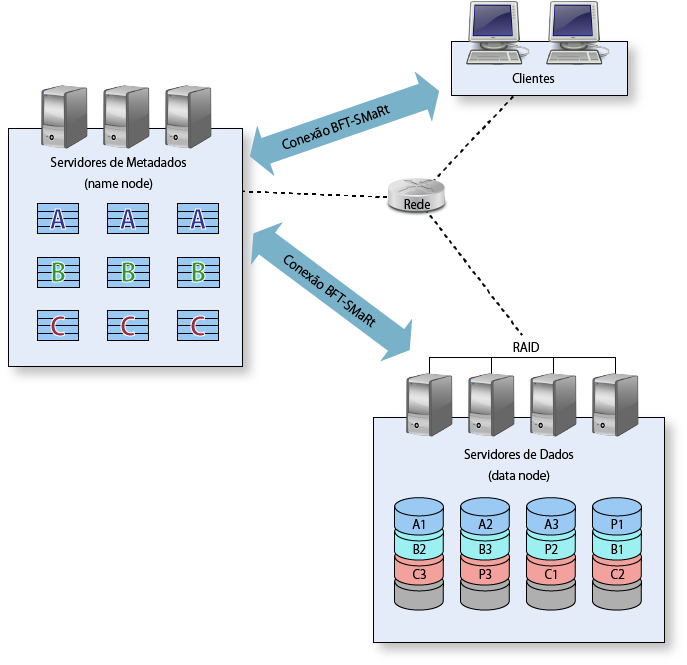
\includegraphics[width=\textwidth]{imagens/visao_geral}
			%\caption{}
		\end{figure}
	\end{columns}
	
\end{frame}


\begin{frame}{Servidor de metadados}
	
	\begin{columns}
		\column{0.55\textwidth}
		\begin{itemize}
			\item Fornece o serviço de metadados.
			\item Protegido pelo BFT-SMaRt com replicação de serviços.
			\item Comunica com os servidores de dados e os clientes através de conexão BFT-SMaRt.
			\item Métodos de comunicação usados: appExecuteOrdered e appExecuteUnordered.
		\end{itemize}
		\column{0.45\textwidth}
		
		\begin{figure}
			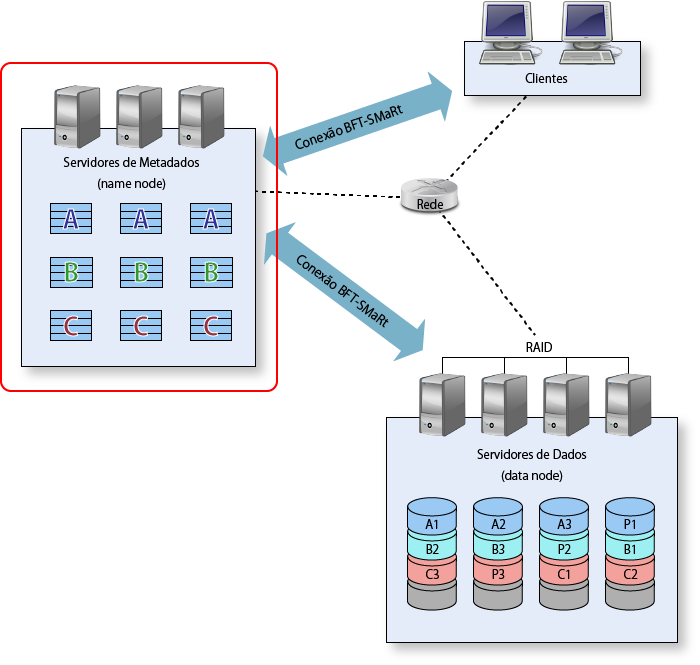
\includegraphics[width=\textwidth]{imagens/visao_geral1}
			%\caption{}
		\end{figure}
	\end{columns}
\end{frame}

\begin{frame}{Servidor de dado}
	
	\begin{columns}
		\column{0.55\textwidth}
		\begin{itemize}
			\item Armazena os arquivo em forma de blocos.
			\item Aplicação de RAID para tolerar as falhas ou aumentar o desempenho.
			\item Comunica com clientes através de conexão Java Socket.
			\item Se comporta como um cliente do sistema BFT-SMaRt.
		\end{itemize}
		\column{0.45\textwidth}
		
		\begin{figure}
			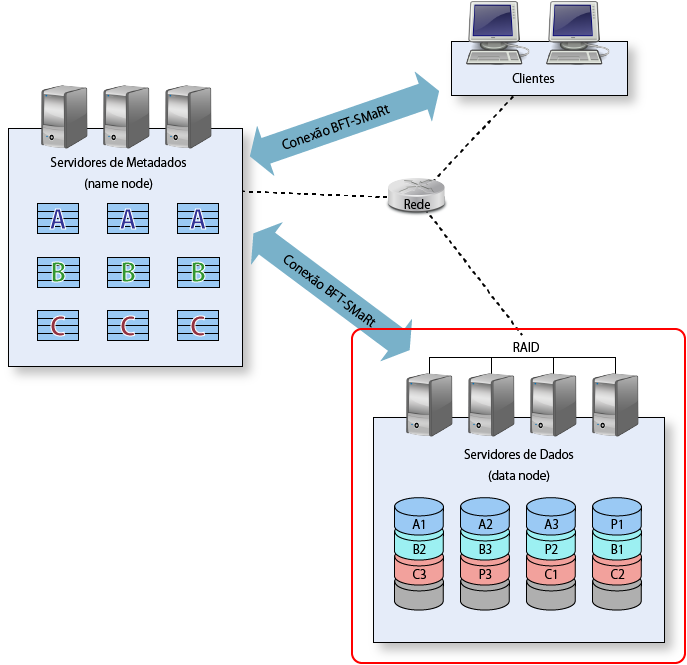
\includegraphics[width=\textwidth]{imagens/visao_geral2}
			%\caption{}
		\end{figure}
	\end{columns}
\end{frame}


\begin{frame}{Cliente}
	\begin{columns}
		\column{0.55\textwidth}
		\begin{itemize}
			\item Interface com os usuários.
			\item Preparação de arquivo para envio: partição e geração de paridades.
			\item Método para requisição: invokeOrdered e invokeUnordered.
		\end{itemize}
		\column{0.45\textwidth}
		
		\begin{figure}
			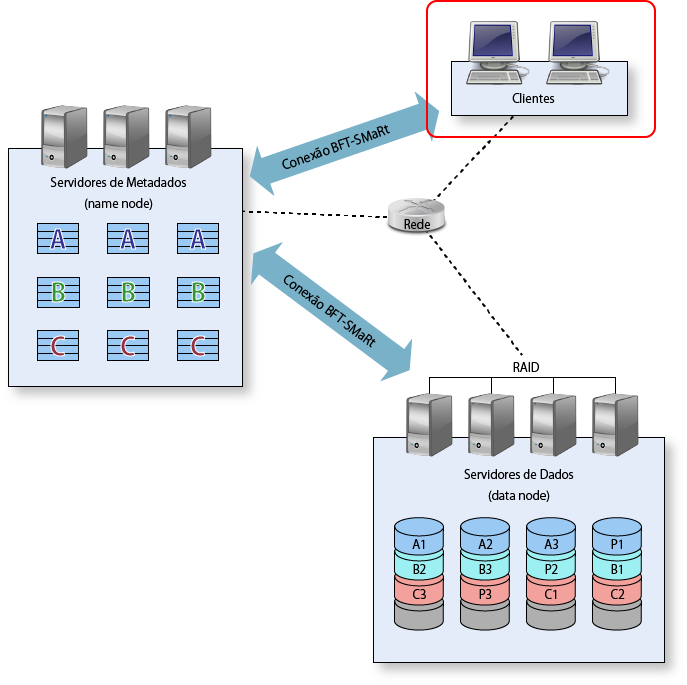
\includegraphics[width=\textwidth]{imagens/visao_geral3}
			%\caption{}
		\end{figure}
	\end{columns}
	
\end{frame}


